\documentclass{article}
\usepackage[utf8]{inputenc}
\usepackage[spanish]{babel}
\usepackage{graphicx}
\usepackage{textcomp}
\usepackage{blindtext}
\usepackage{textpos}
\usepackage{float}
\usepackage{hyperref}

\begin{titlepage}
        \centering
        
\includegraphics[width=9.5cm]{img/Logo TEC.png}\\[1cm]
        {\scshape\LARGE\bfseries  Instituto Tecnológico de Costa Rica \par}
        \vspace{2cm}
        {\scshape\LARGE\bfseries  Lenguajes de Programación\par}
        \vspace{2cm}
        {\scshape\LARGE\bfseries  Profesor Eddy Ramírez\par}
        \vspace{2cm}
        {\scshape\LARGE\bfseries  Cuarto Proyecto Programado\par}
        \vspace{2cm}
        {\scshape\LARGE\bfseries  Sebastián Solórzano Guzmán\par}
        \scshape\LARGE\bfseries 2016138505\par
        \vspace{2cm}
        {\scshape\LARGE\bfseries  Christian Acuña Sáenz\par}
        \scshape\LARGE\bfseries 2013038916\par
        \vspace{2cm}
        \vfill
        {\large \today\par}
        
\end{titlepage}

\begin{document}


\section{Resumen Ejecutivo} 
En este caso nuestro Programa Inicia y se detiene correctamente, crea los sockets y los hilos por jugador para que se mantenga la conexión abierta, también se logro crear el modulo cliente; el cual lastimosamente no imprime todas las cartas de los jugadores en la sección pero tiene la capacidad de poder con el objeto carta el cual tiene a disponibilidad los recursos de imagen aportados por el profesor Eddy Ramírez, en el caso del servidor trata de iniciar el juego pero como los juegos no pudieron ser implementados en un 100 por ciento, no logra continuar con la lógica para que los clientes funcionen lo cual mantiene en un ciclo infinito o cierra conexión.

\newpage
\section{Introducción}
El póquer (o póker) es un juego de apuestas en el que los jugadores, con todas o parte de sus cartas ocultas, hacen apuestas sobre una puja inicial, recayendo la suma total de las apuestas en el jugador o jugadores con la mejor combinación de cartas.
\\
La historia del póquer es un tema de debate. El nombre del juego parece provenir del término francés poque, que desciende a su vez del alemán pochen (golpear), pero no está claro si los juegos a los que se refieren estos nombres fueron los verdaderos orígenes del póquer. Tiene una gran similitud con el juego persa as nas, y puede que los marineros persas se lo enseñasen a los colonos franceses en Nueva Orleans. Se cree que comparte paternidad con el antiguo juego del Renacimiento llamado primero y con el francés "blean".
\\
El juego inglés brag (del antiguo bragg), descendía claramente de brelan, e incorporó el bluffing “engaño, farol” (aunque el concepto ya era conocido en otros juegos de aquella época). Es bastante posible que todos estos juegos antiguos influyeran en el desarrollo del póquer tal y como existe en la actualidad.
\\
El juego y jerga del póquer han llegado a ser parte importante de las culturas de habla inglesa. Frases como ace in the hole (un as en la manga), beats me (ni idea), blue chip (de primera), call the bluff (ver un farol, darse cuenta de que alguien farolea), cash in (sacar partido), poker face (poner cara de póquer, refiriéndose a no mostrar expresión alguna en el rostro), stack up (adelantarse), wild card (carta comodín o joker) y otras, son usadas en conversaciones cotidianas, incluso fuera de su contexto de la mesa de póquer.
\\
El torneo moderno se hizo popular en los casinos estadounidenses tras el comienzo de las Series Mundiales de Póquer en 1970. Fue también durante esta década cuando aparecieron los primeros libros serios acerca de estrategia; en particular Theory of Poker, por David Sklansky; o Super system, por Doyle Brunson. Las retransmisiones vía satélite y por cable de los torneos han añadido popularidad al juego.
\newpage
\section{Descripción de la solución}
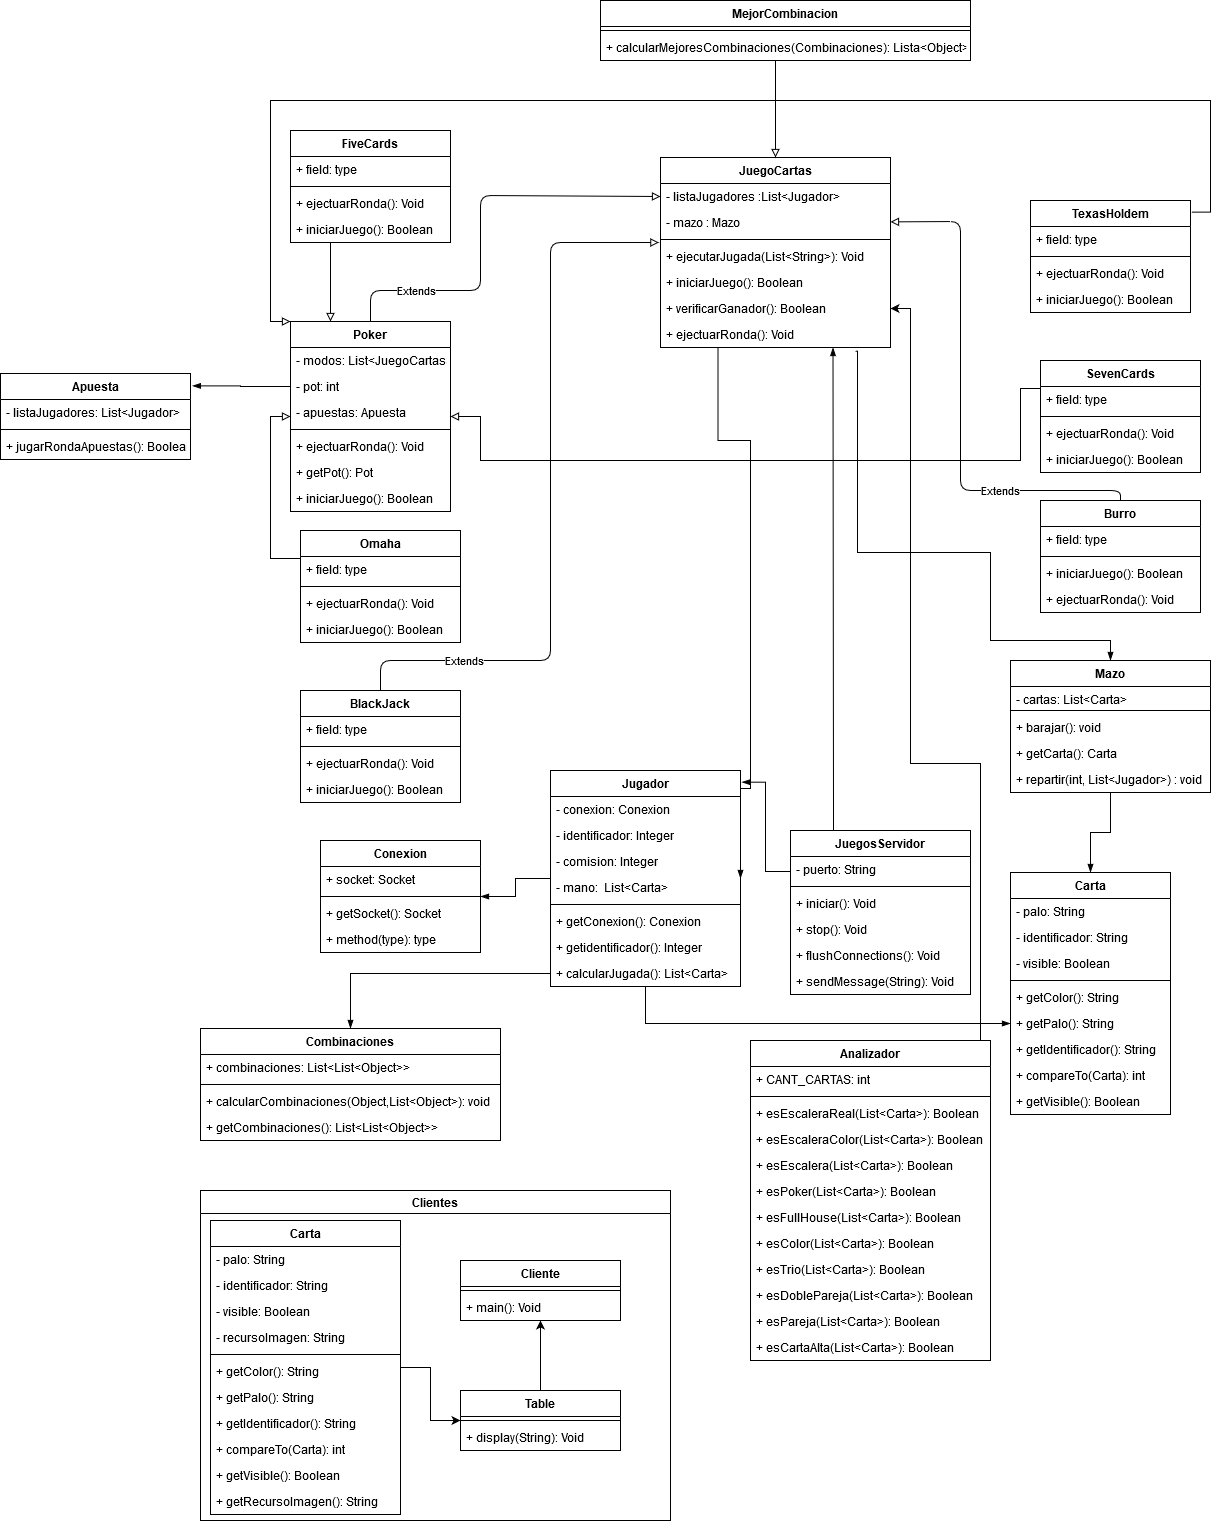
\includegraphics[width=9.5cm]{img/Diagrama de Clases.png}\\[1cm]
Se hace uso de una clase JuegoCartas que proporciona la base de cualquier juego de cartas que se quiera implementar y por medio de herencia se crea el póker en concreto, que cuenta más clases hijas que representan los diferentes modos de juego que se pueden jugar en un juego de póker.
\\\\
Se crean clases básicas para cualquier juego de cartas como pueden ser Carta y Mazo que proporcionan la funcionalidad, que harán la representación de estos objetos de la vida real dentro de nuestro programa con características esperadas como por ejemplo el palo, numero y color de la carta y funcionalidades como barajar, repartir y obtener carta del mazo.
\\\\
Se representa también el jugador en una clase que posee información como la mano del jugador, representada como una lista de cartas y la cantidad de dinero con la que cuenta el jugador para hacer las apuestas y otras funciones relacionadas a la conexión con el servidor para poder jugar. Para la definición de las jugadas y así determinar un ganador se implementa una clase Analizador que se encarga de analizar una combinación de cinco cartas, las cuales serían la jugada de un jugador, para determinar que tipo de jugada es y así poder comparar las diferentes manos para declarar un ganador.
\\\\
Para determinar la jugada de un jugador se diseñan dos clases, Combinaciones y MejorCombinacion. Combinaciones se encarga de listar todas las combinaciones posibles que tiene un jugador con las cartas que tiene en mano y las cartas que se reparten en la mesa. MejorCombinacion se encarga de tomar todas las combinaciones encontradas y determinar cual es la mejor haciendo uso de Analizador para escoger la mejor jugada posible.
\\\\
Para poder iniciar el servidor se ocupa una clase, JuegosServidor, la cual es encargada de escuchar por socket las conexiones y crear jugadores conforme clientes se vayan uniendo, una vez obtenido la cantidad de jugadores deseada se iniciar con el juego creando la una clase de JuegoCartas de tipo deseado.
\\\\
Para la sección de cliente, se tiene 3 clases, la clase Cliente que tiene como objetivo tener una conexión directa con el servidor, la clase Carta la cual tiene toda la información necesaria para poder mostrarse en la clase Tabla, la cual se encarga de mostrar una Tabla donde están todas las cartas de los jugadores, en que posición y las cartas de la mesa.
\newpage



\section{Justificación del Diseño}
Primero pensamos en la clase JuegoCartas, la cual debería ser la clase padre de todos los juegos de cartas que se van a implementar, de ahí pudimos deducir que Poker, Burro y BlackJack pueden extenderse de JuegoCartas, en el caso de Poker que puede tener como hijos los juegos, Omaha, SevenCards, FiveCards y TexasHold'em, teniendo seleccionados todos los juegos requeridos para el proyecto, empezamos a sacar las sub-partes de cada objeto(Atributos/Métodos) en caso de JuegoCartas, para ser un Juego de cartas, se debería tener un objeto Carta, el cual como atributo se puede saber el identificador, el palo y si es visible o no; este ultimo ya que hay juegos donde se requiere que la carta no sea visible por el jugador asta cierto momento en el juego. También pudimos observar que los juegos de cartas tienen Mazo el cual es una Lista de cartas la cual se encarga de poder barajarse y de poder repartir las cartas a los jugadores, y con esto podemos también observar que JuegosCartas tienen un objeto de MejorCombinaciones, el cual se encarga de obtener la MejorCombinacion de una combinación cualquiera y también JuegoCartas debería saber cuando alguien debería ganar, por lo cual tiene un Objeto Analizador el cual le dice si tiene un grupo predeterminado de cartas y cual seria ese grupo.
\\\\
Como se puede observar se debe implementar un modelo cliente servidor el cual permitirá a los jugadores jugar por medio de Sockets sobre la red, para eso seria la clase Juegos Servidor la cual tiene como encargado obtener la información de los Jugadores; específicamente el tipo de conexión, y de enviar a los clientes el tipo de juego que se va a jugar, para eso tenemos una clase Jugador la cual se especializa en guardar los datos del jugador, como es la mano, identificador y la Conexión, la cual sera usada por el mazo para repartir las cartas.
\newpage
\section{Resultados y Pruebas} 
En caso de que el cliente trate de conectarse pero el servidor no se encuentre disponible.
\\\\
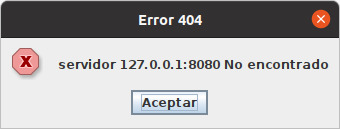
\includegraphics[width=9.5cm]{img/pba1.jpeg}\\[1cm]
En esta prueba es en el caso de que el juego haya terminado o el servidor terminara la conexión.
\\\\
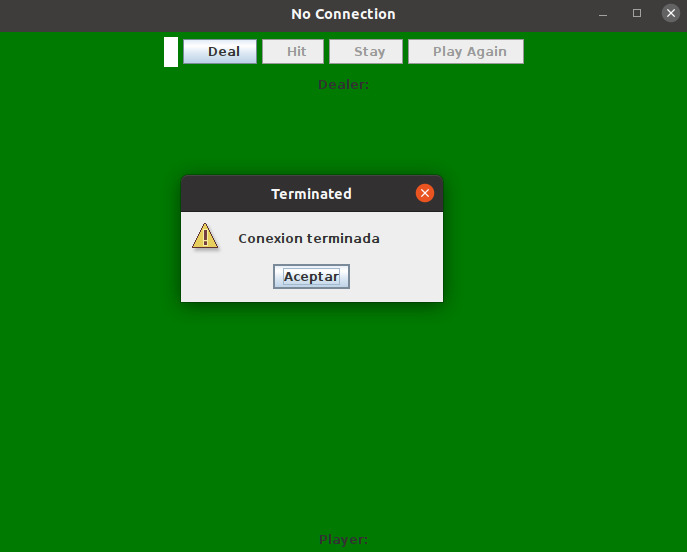
\includegraphics[width=9.5cm]{img/pba2.jpeg}\\[1cm]

\newpage
\section{Conclusiones}

Se concluye que para utilizar lenguajes orientados a Programación de Objetos Java es muy especializado en ese tema, casi que es la herramienta "go-to" de los programadores, para este proyecto se nos facilito primero hacer el diseño de clases, lo cual repercutió que la mayoría del trabajo saliera fácilmente, lastimosa mente nuestro diseño no estaba 100 por ciento completado, ya que conforme fuimos programando, empezamos a ver que pudimos agregar o eliminar clases que no eran necesarias, lo cual llego a un momento donde nos tuvimos que parar y volver a pensar el diseño.
\\
\\
\newpage
\section{Reflexión de lo aprendido}

Sebastián: Es interesante ver la importancia del diseño para trabajar en programación orientada a objetos y lo fácil que se vuelve la implementación de una solución cuando se tiene un buen diseño. En este proyecto el lenguaje no presenta un problema ya que he tenido la posibilidad de trabajar en este antes, lo mismo con el paradigma, sin embargo, no es hasta ahora que me doy cuenta del tiempo que se le debe dedicar a la parte de modelaje comparado a la implementación si se quiere que esta última sea más sencilla.
\vspace{0.5cm}\\
Christian: Fue interesante volver a tocar Java después de varios años, pero me di cuenta lo versátil que se siente comparado con los proyectos pasados, ya que me tengo que preocupar mas por como buscar cosas que me puedan servir en el docs y de como implementar un diseño correcto que el algoritmo en si, pero lo bueno es que hay mucha mucha mas documentación sobre Java que de los proyectos pasados, mi recomendación es que primero busque ejemplos de código de Java para que se familiarice un poco mas con el y siempre tener una ventana de java docs para guiarse, aparte de eso siempre tener disponible alguna herramienta o IDE que te ayuda a programar de manera mas rápida y que pueda organizar el código ya que la cantidad de código que se escribe es mucho comparado con los proyectos pasados que fueron en C,Erlang y Prolog.
\newpage
\section{Bibliografía}

*Póquer. (s.f.). Accesado el 18 de Agosto de 2020. Recuperado de:
\url{https://es.wikipedia.org/wiki/Poquer}.
\\
\\
*BlackjackDemo. (s.f.). Accesado el 10 de Agosto de 2020. Recuperado de:
\url{https://faculty.washington.edu/moishe/javademos/blackjack/}.
\end{document}
